\documentclass[hidelinks, 12pt, a4paper]{article}

\usepackage{tabularx} %full-width tables
\usepackage{moresize} %Huge and HUGE
\usepackage[margin=0in]{geometry}%Margins
\usepackage[none]{hyphenat}%Remove hyphenation
\usepackage{enumitem}%to set gaps in itemize
\usepackage{fontawesome}
\usepackage{hyperref}
\usepackage{blindtext}
\usepackage{xcolor}
\usepackage{afterpage}
\usepackage{tikz}
\usepackage[skins]{tcolorbox}

\usepackage{multicol}

\usepackage[sfdefault,light]{roboto}

%\cellwidth in tabularx size
\makeatletter
\newcommand\cellwidth{\TX@col@width}
\makeatother

\definecolor{sidebarColor}{HTML}{001C5E}
\definecolor{skillBackground}{HTML}{98A0B2}
\definecolor{skillForeground}{HTML}{EBA500}

%Right-aligned tabularx
\newcolumntype{R}{>{\raggedleft\arraybackslash}X}

%No page numbering
\pagenumbering{gobble}

\newcommand{\smitem}[1]{\item {\small {#1}}}

\newenvironment{bullets}{\begin{minipage}[t]{\linewidth}\begin{itemize}[leftmargin=2em,label=-,nosep]}{\end{itemize}\end{minipage}\vspace{5pt}}

\newenvironment{sectionitem}{\vspace{6pt}\noindent\tabularx{\linewidth}{p{70pt}X}}{\endtabularx}


\newcommand{\sectionheader}[1]{
	\vspace{6pt}
	{
		\noindent
		\hspace{3pt}
		%\fontfamily{lmr}\selectfont
		\Large\textbf{#1}}}

\begin{document}
		\noindent\fcolorbox{sidebarColor}{sidebarColor}{%
			\color{white}
			\begin{minipage}{\dimexpr0.35\textwidth-2\fboxrule-2\fboxsep\relax}
				\vspace{4pt}
				\begin{center}
					\begin{tikzpicture}
						\color{black}
						\node[circle,draw,inner sep=40pt,fill overzoom image=picture] (A) {};
					\end{tikzpicture}\\
					\vspace{12pt}
					\textbf{
						\LARGE Steven Lowes
					}
				\vspace{8pt}
				
				\begin{tabular}{rc}
					\href{https://www.google.co.uk/maps/@54.7840735,-1.5497025,14z}{Durham, UK} & \href{https://www.google.co.uk/maps/@54.7840735,-1.5497025,14z}{\faHome}\\
					\href{mailto:steven@stevenlowes.com}{steven@stevenlowes.com} & \href{mailto:steven@stevenlowes.com}{\faEnvelope}\\
					0737 843 8686 & \faPhone \\
					\href{https://www.linkedin.com/in/steven-lowes/}{steven-lowes} & \href{https://www.linkedin.com/in/steven-lowes/}{\faLinkedin} \\
					\href{https://github.com/motherlymuppet}{motherlymuppet} & \href{https://github.com/motherlymuppet}{\faGithub} \\
					\href{http://www.stevenlowes.com}{stevenlowes.com} & \href{http://www.stevenlowes.com}{\faLink} \\
				\end{tabular} \\
			
			\vspace{12pt}
				\textbf{
					\Large Summary
				}
		
				\vspace{8pt}
				\begin{minipage}{0.9\linewidth}
					Second year Computer Science student at Durham University. Excellent problem solver, willing to take time to ensure a solution is optimal. Self-directed and efficient, able to learn new technologies quickly. Proficient public speaker with great communication in teams.
				
					\vspace{8pt}
					
					Extensive experience with Java and SQL. Experience with full-stack web development, desktop application development, database creation and administration.
					
					\vspace{8pt}
					
					Interested in working on large applications, where scalability and extensibility are priorities.
				\end{minipage}
			
				\vspace{16pt}
				
				\textbf{
					\Large Skills
				}
			
		
			\vspace{4pt}
			
\begin{tikzpicture}
				\node [anchor=west,rotate=90] at (0,0.25) {};
				\node [anchor=west,rotate=90] at (1.26,0.25) {\textbf{Beginner}};
				\node [anchor=west,rotate=90] at (2.62,0.25) {\textbf{Competent}};
				\node [anchor=west,rotate=90] at (3.98,0.25) {\textbf{Skilled}};
				\node [anchor=west,rotate=90] at (5.34,0.25) {\textbf{Advanced}};
				\node [anchor=west,rotate=90] at (6.55,0.25) {\textbf{Expert}};
			\end{tikzpicture}
			
			
\begin{tikzpicture}
				\fill [skillBackground] (0,0) rectangle(6.8,.5);
				\fill [skillForeground] (0,0) rectangle(5.44,.5);
				\node [anchor=west] at (.1,0.25) {\textbf{Java}};
			\end{tikzpicture}

			\vspace{4pt}
			
\begin{tikzpicture}
				\fill [skillBackground] (0,0) rectangle(6.8,.5);
				\fill [skillForeground] (0,0) rectangle(5.44,.5);
				\node [anchor=west] at (.1,0.25) {\textbf{SQL}};
			\end{tikzpicture}

			\vspace{4pt}
			
\begin{tikzpicture}
				\fill [skillBackground] (0,0) rectangle(6.8,.5);
				\fill [skillForeground] (0,0) rectangle(4.08,.5);
				\node [anchor=west] at (.1,0.25) {\textbf{Javascript}};
			\end{tikzpicture}
			
			\vspace{4pt}
			
\begin{tikzpicture}
				\fill [skillBackground] (0,0) rectangle(6.8,.5);
				\fill [skillForeground] (0,0) rectangle(4.08,.5);
				\node [anchor=west] at (.1,0.25) {\textbf{Git}};
			\end{tikzpicture}
			
			\vspace{4pt}
			
\begin{tikzpicture}
				\fill [skillBackground] (0,0) rectangle(6.8,.5);
				\fill [skillForeground] (0,0) rectangle(4.08,.5);
				\node [anchor=west] at (.1,0.25) {\textbf{Technical Writing}};
			\end{tikzpicture}
			
			\vspace{4pt}
			
\begin{tikzpicture}
				\fill [skillBackground] (0,0) rectangle(6.8,.5);
				\fill [skillForeground] (0,0) rectangle(4.08,.5);
				\node [anchor=west] at (.1,0.25) {\textbf{Python}};
			\end{tikzpicture}
			
			\vspace{4pt}
			
\begin{tikzpicture}
				\fill [skillBackground] (0,0) rectangle(6.8,.5);
				\fill [skillForeground] (0,0) rectangle(2.72,.5);
				\node [anchor=west] at (.1,0.25) {\textbf{Unit Testing}};
			\end{tikzpicture}
			
			\vspace{4pt}
			
\begin{tikzpicture}
				\fill [skillBackground] (0,0) rectangle(6.8,.5);
				\fill [skillForeground] (0,0) rectangle(2.72,.5);
				\node [anchor=west] at (.1,0.25) {\textbf{Agile}};
			\end{tikzpicture}
			
			\vspace{15pt}
			\end{center}
		\end{minipage}
	}
	\hspace{0.02\textwidth}
	\begin{minipage}{0.6\textwidth}
		\sectionheader{Education}
		
		\begin{sectionitem}
			2016 --- 2019&\textbf{\href{https://www.dur.ac.uk/}{Durham University}} (\href{https://www.dur.ac.uk/trevelyan.college/}{Trevelyan College})\\
			\emph{Durham}&\href{https://www.dur.ac.uk/courses/info/?id=11509\&title=Computer+Science\&code=G400\&type=BSC\&year=2016}{Bsc Computer Science}\\
			&\begin{bullets}
				\smitem{Year 2: On Track for \textbf{81\%}}
				\smitem{Year 1: \textbf{74\%} overall, \textbf{77\%} in CompSci Modules}
			\end{bullets}
		\end{sectionitem}
	
		\begin{sectionitem}
			2015 --- 2016&\textbf{\href{https://www.dur.ac.uk/}{Durham University}} (\href{https://www.dur.ac.uk/trevelyan.college/}{Trevelyan College})\\
			\emph{Durham}&\href{https://www.dur.ac.uk/courses/info/?id=11558\&title=General+Engineering\&code=H100\&type=MENG\&year=2015}{MEng General Engineering}\\
			&\begin{bullets}
				\smitem{Year 1: 2:2 Equivalent}
				\smitem{Module - \href{https://www.dur.ac.uk/faculty.handbook/module_description/?module_code=COMP1011}{\emph{Introduction to Programming}: \textbf{89\%}}}
			\end{bullets}\\
			&Switched to the Computer Science Degree after discovering my love for programming\\
		\end{sectionitem}
		
		\begin{sectionitem}
			2013 --- 2015&\textbf{\href{http://www.parkviewlearning.net/post-16-education/sixth-form/}{Park View Sixth Form}}\\
			\emph{Co. Durham}&A-Level Grades:\\
			&\begin{bullets}
				\smitem{Business Studies - A*}
				\smitem{Maths - A}
				\smitem{Physics - B}
			\end{bullets}\\
		\end{sectionitem}
		
		\begin{sectionitem}
			2008 --- 2013&\textbf{\href{http://www.parkviewlearning.net/}{Park View School}}\\
			\emph{Co. Durham}&GCSE Grades:\\
			&\begin{minipage}[t]{\linewidth}\begin{multicols}{4}\begin{description}[nosep]
						\item 3 $\times$ A*
						\item 6 $\times$ A
						\item 1 $\times$ B
						\item 1 $\times$ C
					\end{description}
				\end{multicols}
			\end{minipage}
		\end{sectionitem}
	
		\sectionheader{Work}
		
		\begin{sectionitem}
			March ---&\textbf{Full Stack Developer}\\
			May 2017&\href{http://planforprobate.com/}{Plan for Probate (North) Ltd.}\\
			\emph{Co. Durham}&\begin{bullets}
				\smitem{Developed an online portal to store client information and track payments}
				\smitem{Employed Agile methodologies to keep the owners updated and work to the evolving requirements}
				\smitem{Technologies Used: Java, JSP, Bootstrap, SQL, Javascript, Google Cloud Services}
			\end{bullets}\\
		\end{sectionitem}
		
		\begin{sectionitem}
			July ---&\textbf{Java Desktop Application Programmer}\\
			Oct 2016&\href{https://www.facebook.com/tripefactory.sunderland/}{E. Hall Tripe \& Poultry Ltd.}\\
			\emph{Sunderland}&\begin{bullets}
				\smitem{Worked from a brief to develop a logistics system for the factory}
				\smitem{The program tracked orders and repeat orders, creating lists of products for the delivery drivers}
				\smitem{The program organised routing for the deliveries, which was previously done by hand}
				\smitem{Technologies Used: Java, Swing, SQL}
			\end{bullets}\\
		\end{sectionitem}
		
		\begin{sectionitem}
			2013 ---&\textbf{Desktop Application Developer}\\
			Present&\href{http://www.lowes.co.uk}{Lowes Financial Management}\\
			\emph{Newcastle}&\begin{bullets}
				\smitem{Created and maintained various tools which analyse financial products}
				\smitem{The tools produce graphs and data which are used in literature distributed to clients and have been published in online articles by Lowes}
				\smitem{Technologies Used: Java, SQL, Excel, VBA}
			\end{bullets}\\
		\end{sectionitem}
	
		\sectionheader{Student Groups}
		\vspace{4pt}
		
		President of Code Wars society. Involved in DU Robot Wars team. Actively involved with \href{http://community.dur.ac.uk/dur.improv/}{ShellShock! Improvised Comedy}. Elected to sit on Societies Committee which governs other student groups. Elected as Course Rep and Co-Chair of the Student-Staff Committee.
	\end{minipage}

	\newpage
	
	\vspace*{12pt}
	
	\begin{center}
		\Huge Portfolio
	\end{center}
	
	\hspace{0.02\textwidth}
	\begin{minipage}{0.40\textwidth}		
		\begin{center}
			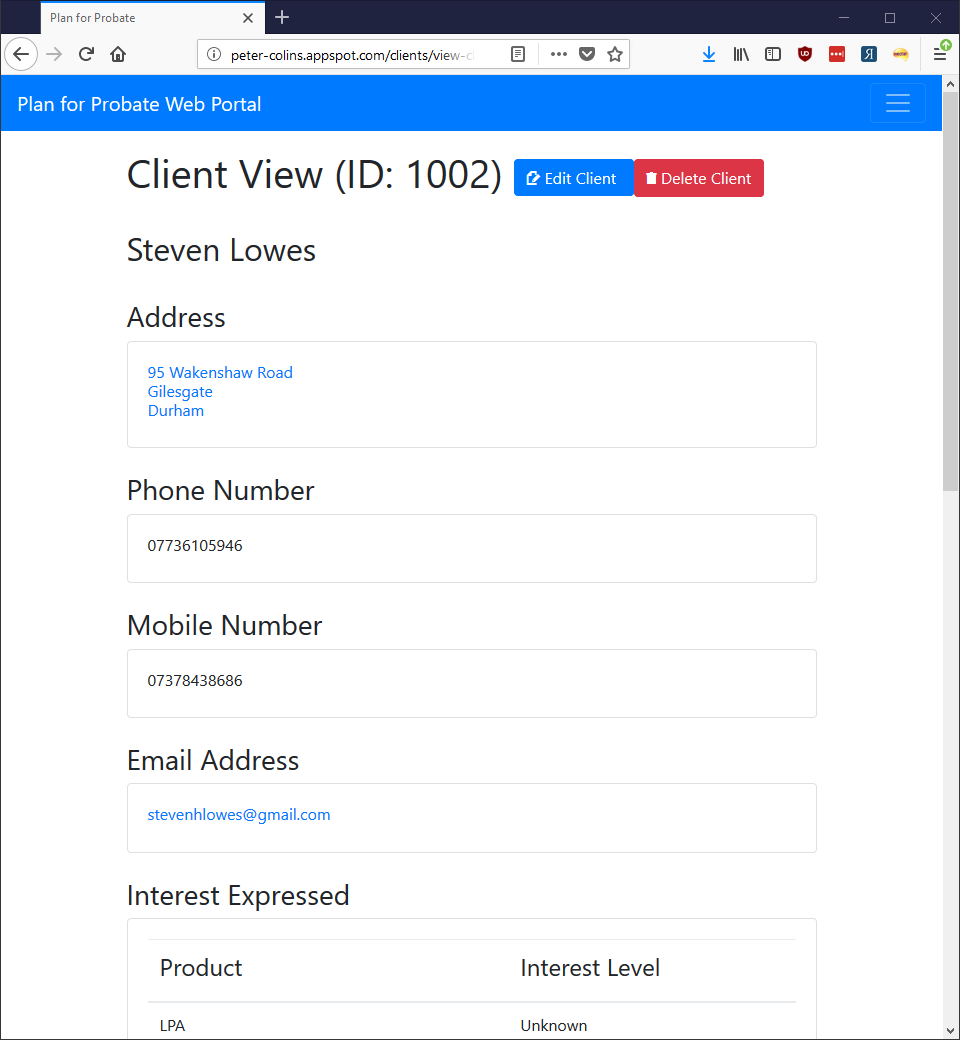
\includegraphics[width=0.9\linewidth]{planforprobate.png}
		\end{center}
		\vspace{-12pt}
		\textbf{Plan For Probate Web Portal} (May 2017)
		
		Plan For Probate's internal web portal. Tracks clients, and tasks currently in progress. Allows for file upload and storage for important documents. Secured using Google Login, and Database encrypted to comply with GDPR. Used by the company to store and manage all ongoing tasks and client information. The web portal has replaced the previous system which used index cards to track their clients. The web portal significantly decreased the time spent on admin and numer of errors/missed appointments.
		
		\textbf{Technologies Used:} Java, SQL (MySQL), JSP, Bootstrap, Javascript, Google Cloud Platform
		
		\begin{center}
			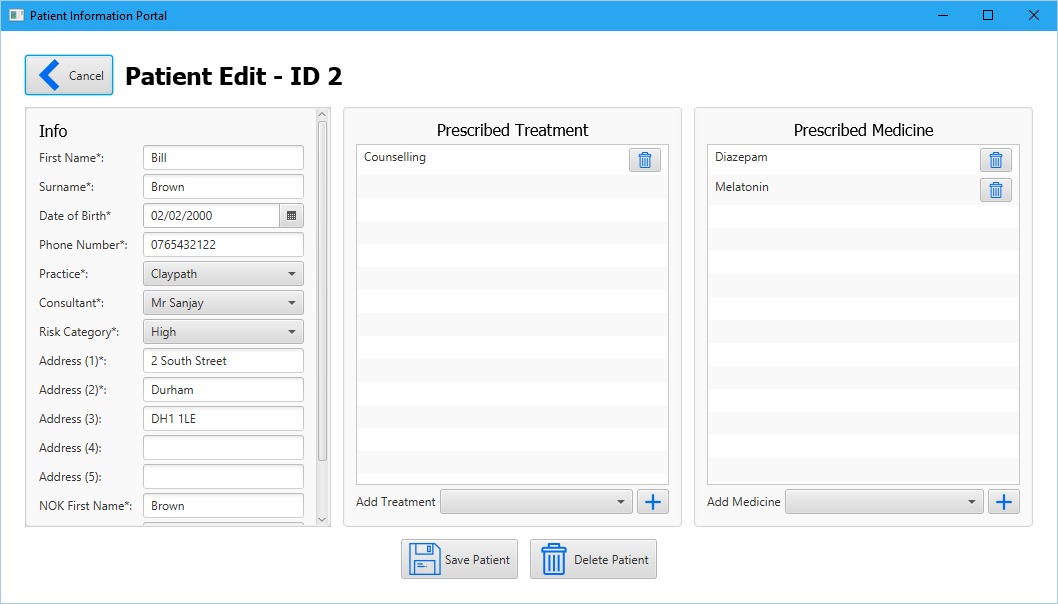
\includegraphics[width=0.9\linewidth]{sarahassignment.png}
		\end{center}
		\vspace{-12pt}
		\textbf{Patient Information Portal} (Feb 2018)
		
		University Assignment. Focussed on creating GUIs following principles of Human-Computer Interaction. Used the opportunity to learn JavaFX to replace Swing. Backed by a remote MySQL Database and a DAO layer. The mark for this assignment is still pending.
		
		\textbf{Technologies Used:} SQL (MySQL), Java, JavaFX
		
	\end{minipage}
	\hspace{0.06\textwidth}
	\begin{minipage}{0.40\textwidth}
		
		\begin{center}
			\href{http://www.dsurooms.com}{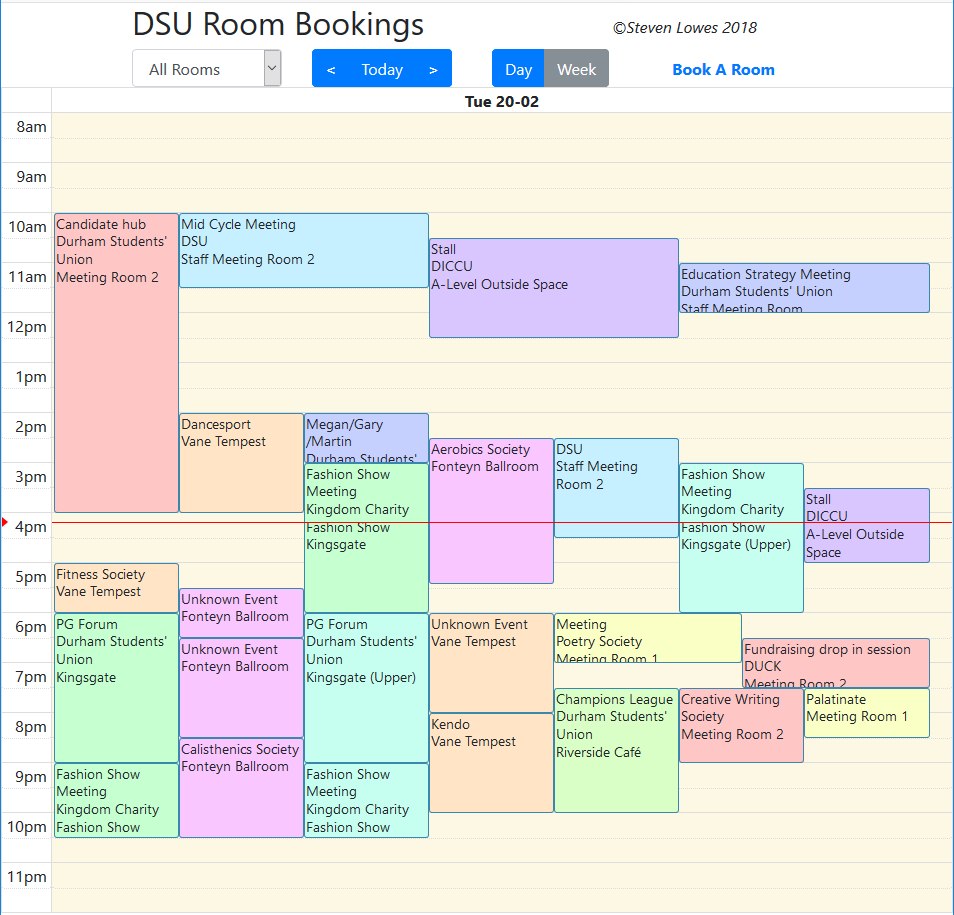
\includegraphics[width=0.9\linewidth]{dsurooms.png}}
		\end{center}
		\vspace{-12pt}
		\href{http://www.dsurooms.com}{\textbf{DSUrooms.com} (Jan 2018)}
		
		Created for Societies Committee, to show when rooms in the Students' Union were booked. Received very positive feedback from Student Groups, as previously there was no way to know which rooms were booked. Not yet in full release, but in use by a small group of executive committees.
		
		\textbf{Technologies Used:} NodeJS, FullCalendar, Javascript, JQuery, RedHat Openshift
		
		\begin{center}
			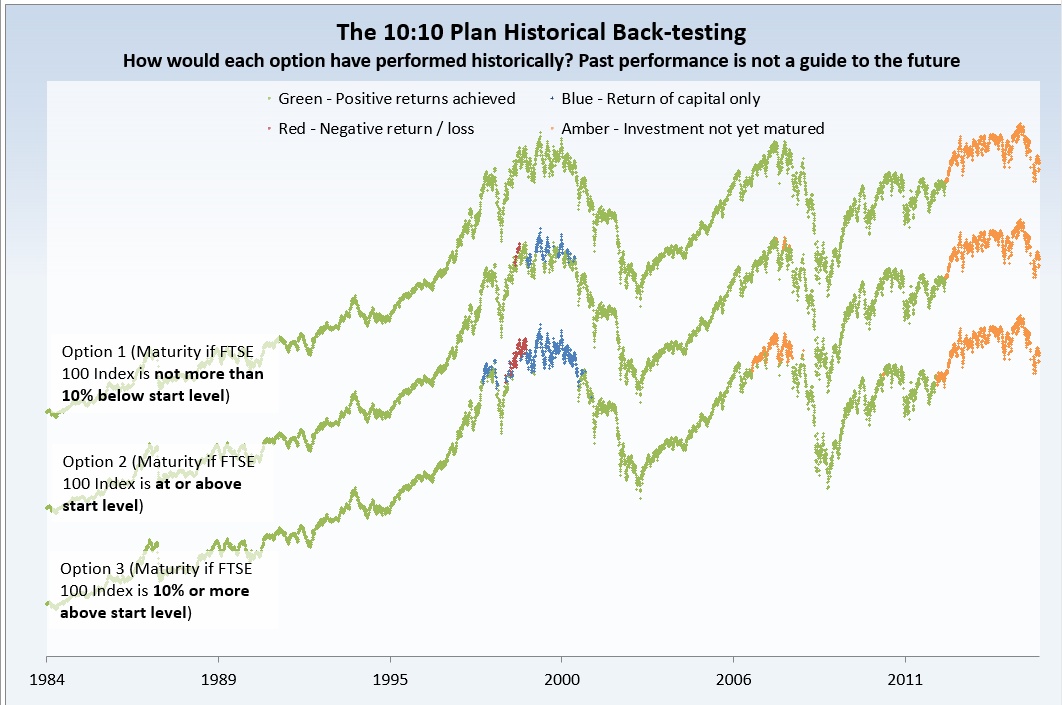
\includegraphics[width=0.9\linewidth]{backtest.png}
		\end{center}
		\vspace{-12pt}
		\textbf{Autocall Backtester} (March 2016)
		
		Created for Lowes Financial Management. Tests a financial product to see how it would have performed historically. This tool allowed the analysis to be performed where previously it was too time consuming. The graphs produced are used in the official product literature and online. The tool also informed the creation of new products, where backtesting revealed them to perform better than expected.
		
		\textbf{Technologies Used:} Java, Excel
	\end{minipage}
	\hspace{0.02\textwidth}
	
	
\end{document}